\part{Sleep Detection}

    \chapter{Overview}

        This section covers the development and evaluation of the sleep detection algorithm. The algorithm aims to extract features like sleep onset time, wakefulness onset time, and total time asleep from accelerometer data recorded on a wrist-mounted device.

        The basis of this algorithm relies on the fact that the level of activity of a person can be determined from the magnitude of the standard deviation or the energy of the accelerometer signal. If there is no movement, the standard deviation should be the square root of the variance of the noise in the accelerometer sensor (assumed to be zero-mean Gaussian). If there is a high level of movement, then there will be a high standard deviation from the signal. If there is a long period of low activity then this period will be defined as asleep. This set of rules and inferences will be the guiding principles upon which the algorithm is built.

        All of the data used in the algorithm development and validation was analysed at 10Hz.


    \chapter{Database}
        \label{c-database}

        The algorithm development and testing the following chapter relies heavily on a database created by Borazio, et. al. at TU Darmstadt [CIT]. The database contains accelerometer data from 42 patients, their clinically annotated polysomnography results, and light sensor data from overnight stays in a sleep lab. The accelerometer data comes from a custom device that is mounted on the wrist of the patient. The data is logged at 100Hz. 

        The data provided is contained and compressed in such a way that requires reformatting for the use described below. Each patient record has its own file (a .npy file, used for Numpy calculations in Python) which contains 7 columns: a timestamp, the runlength encoding, x-acceleration, y-acceleration, z-acceleration, light sensor value, and a ground truth value. The runlength encoding represents how many times in a row does the following set of measurements repeat, for example runlength encoding of $10$ represents 10 sequential copies of this row with increasing timestamps. All of the acceleration data is stored in an 8-bit unsigned int, from 0 to 255. According to Borazio, et. al. this should map to $-4g$ to $4g$, where $g$ is gravity. The light sensor value is not used in this project and as such will be disregarded. The ground truth is marked as follows: 0 indicates unknown sleep state, 1-3 maps to different sleep states rated from deepest to lightest, 5 indicates random eye movement (REM) sleep, 6 indicates awake, and 7 indicates movement.

        In order to format this data better to the needs of this project a few steps were taken:

        \begin{itemize}
            \item The x,y, and z accelerations will be linearly mapped back to $[-4g,4g]$ and the magnitude will be taken.
            \item The light sensor value will be stripped from the data.
            \item The runlength encoding will be decoded and this column shall be redundent and thus removed.
            \item The data will be downsampled to $10Hz$ to conform with the project specifications.
        \end{itemize}

        The downsampling is a simple operation: keep one point out of every 10 after the runtime encoding decoding is complete. Decoding the runlength encoding is equally simple: duplicate the row of $n$ times where $n$ is the runlength encoding for that row.

        \section{Remapping of Acceleration}

            This operation is fairly straightforward: an original value of $127.5$ is remapped to $0g$ and thusly the value of acceleration can be derived from:

            \begin{equation}
                a_n = (a_o - 127.5)*\frac{8*g}{256}
            \end{equation}
            where $a_n$ is the new acceleration value, $a_o$ is the old value of acceleration, and $g=9.81\frac{m}{s^2}$ is gravity. The format that the acceleration was stored in limits the resolution of the each component, but the combination of the components to the magnitude increases the magnitude slightly.

            This approach is validated by ensuring that the magnitude of the signal is gravity or higher, this is true for the dataset hence this approach is appropriate.



    \chapter{Algorithm Description}

        The algorithm works in two stages: the prediction stage and the post-prediction filter.

        \section{Pre-Prediction Filter}

            Originally, the design included a pre-prediction filter, however this was removed as it degraded overall performance. The implementation and explanations for its removal will be explained here.

            This was aimed to take the accelerometer data and remove high frequency noise and spikes from the signal. This is done through a simple moving average filter.

            Hence, the coefficients of the filter are as follows:

            \begin{equation}
                h_k = \frac{1}{N}, 1\leq k\leq N
            \end{equation}
            where $h_k$ is the $k^{th}$ coefficient of the filter and $N$ is the length of the filter.

            The frequency response of this filter can be seen below in Figure \ref{img_pp_filter}. Body movements are generally slow, so the filter effectively removing higher frequency data is permissible in this use case.

            \begin{figure}[h]
                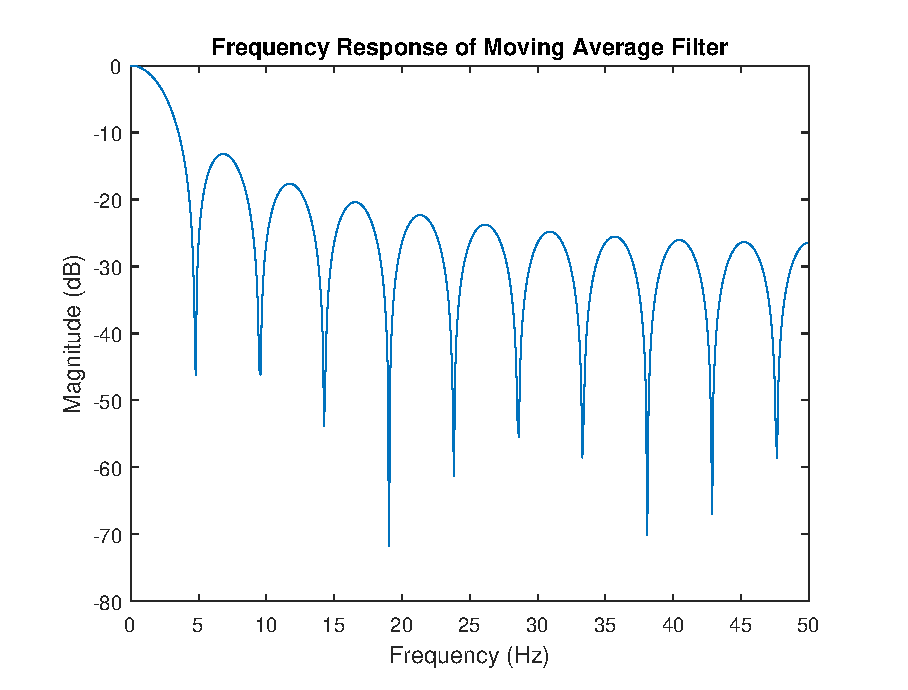
\includegraphics[width=\textwidth]{Images/sleep_pre_filter.eps}
                \centering
                \caption{Frequency response of the pre-prediction filter with a length of 21 samples.}
                \label{img_pp_filter}
            \end{figure}

            An example of the data before filtering and after filtering can be seen below in Figure \ref{img_pp_filter_ex}.

            \begin{figure}[h]
                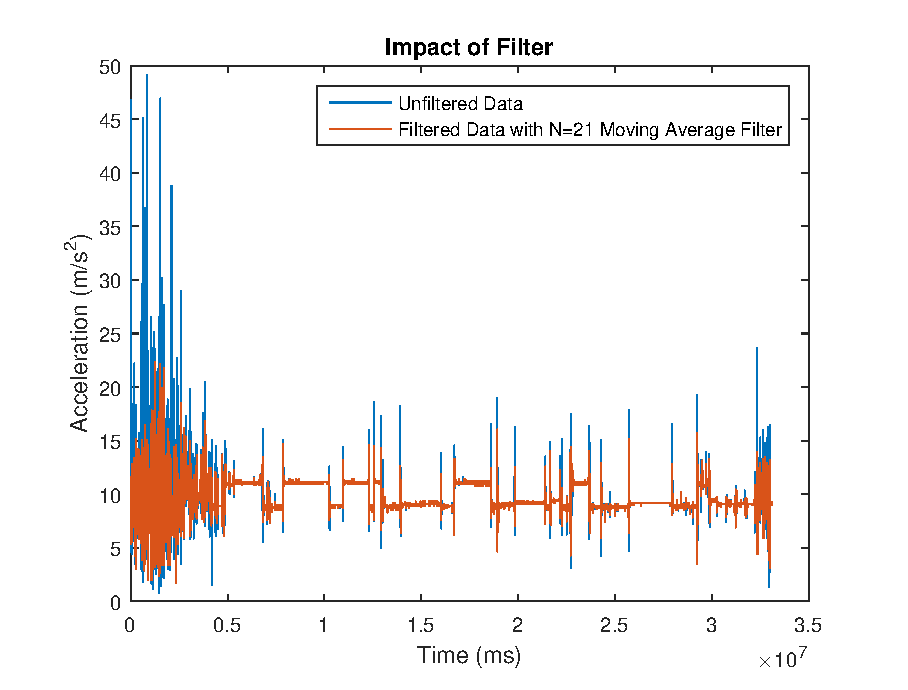
\includegraphics[width=\textwidth]{Images/sleep_pre_filter_ex.eps}
                \centering
                \caption{Example of data before and after filtering. Blue is before filter, orange is after filter. Note the reduced magnitude in the active areas (areas of high magnitude.)}
                \label{img_pp_filter_ex}
            \end{figure}

            However, this graph illustrates why the filter had to be removed. It suppresses areas of high activity thus reducing the standard deviation. This is a direct impact on the quantity that we wish to measure and thus is degrading the information content. Removing the filter increased the algorithm accuracy by around 5\%.           

        \section{Prediction Stage}

            The next stage of the algorithm is to predict whether a chunk of the signal is asleep or awake. The signal is segmented into chunks of 600 samples long, this is equivalent to a period of 1 minute at a 10Hz sampling frequency. This period was chosen as it is close to what one might consider the characteristic length of being asleep. For example, it seems absurd to consider wakefulness on a second by second basis. It also allows for enough information to be captured in the chunk to allow meaningful analysis.

            The prediction is done through a logistic regression, the coefficients of which have been obtained through an optimization process described below in Section \ref{ss_coefficients}.

            The logistic predictor is defined as:

            \begin{equation}
                p(\mathbf{x}, \mathbf{m}) = \frac{1}{1 + e^{-\mathbf{mx}}}
            \end{equation}
            where $\mathbf{x}$ is the feature vector and $\mathbf{m}$ is the coefficient vector. If $p(\mathbf{x}) \geq 0.5$ then that point is classified as asleep (or 1). Otherwise is is classified as awake (or 0).

            \subsection{Coefficients}
                \label{ss_coefficients}

                The feature vector selected for prediction is simple and contains 2 elements: a constant, and the standard deviation. This is defined as follows: 

                \begin{equation}
                    \mathbf{x} = \begin{bmatrix} 1 & \sigma \end{bmatrix}
                \end{equation}

                In order to learn the coefficients, each data segment must have a known ground truth value. That is to say, it is known if the person was awake or asleep during that segment. The database described above was used in acquiring this necessary data. The data was formatted and downsampled like described above in Section \ref{c-database} and then filtered through the moving average filter in the preceeding section. Each data recording was then scanned to look for contiguous periods of sleep or wakefulness. These periods had to be 600 samples long and represented the extremes for a data segment where all of the segment is classified as awake or asleep. These periods were extracted and the feature vector for each was pre-calculated. This dataset would serve as the training and test data for learning the coefficients. 

                In order to optimize the data, a loss function is needed to minimize. This function should encapsulate penalties for incorrect results. 

                To derive this, start with the likelihood of the coefficients given the data:

                \begin{equation}
                    \mathcal{L}(\mathbf{m}) = \prod_{i=1}^n p(y_i|\mathbf{x_i}, \mathbf{m})
                \end{equation}
                where $\mathcal{L}(m)$ is the likelihood of the coefficients, $y_i$ is the ground truth of the $i^th$ data point.

                If the log-likelihood is considered, then this expression can be expanded to:

                \begin{equation}
                    \log{\mathcal{L}(\mathbf{m})} = \sum_{i=1}^n (y_i\log{p(\mathbf{x_i}, \mathbf{m})} + (1-y_i)\log{(1 - p(\mathbf{x_i}, \mathbf{m}))})
                \end{equation}
                where the first term under the summation represents the contribution to the likelihood when $y_i = 1$ and the second term represents the contribution when $y_i = 0$.

                If the log-likelihood is differentiated with respect to $\mathbf{m}$ then it can be shown that the differential is given by:

                \begin{equation}
                    \frac{\partial}{\partial \mathbf{m}}\log{\mathcal{L}(\mathbf{m})} = \sum_{i=1}^n (y_ip(\mathbf{x_i}, \mathbf{m})\mathbf{x_i} - (1-y_i)(1 -p(\mathbf{x_i},\mathbf{m}))\mathbf{x_i})
                \end{equation}

                Unfortunately, this expression has no closed form solution if set to zero (i.e. - if optimizing). In light of this, the logistic regression can only be optimized from methods like gradient descent. The premise of gradient descent is simple, calculate the gradient at a point and then move either up or down the gradient, for maximization and minimization respectively. The downside of this method is that there is no guarantee of getting the global maximum, merely the local maximum. 

                In this project, gradient descent was performed with 200 iterations and a learning rate of $\nu = 0.00004$. Half of the data was used for training and the other half was used for testing. After validating the consistency of the results, the coefficients yielded are given by:

                \begin{equation}
                    \mathbf{m} = \begin{bmatrix} 0.5707 & -2.6377 \end{bmatrix}
                \end{equation}
                where the first coefficient is related to the constant and the second coefficient is related to the standard deviation. The training data had a final accuracy with these coefficients of 72.9\% and the testing data had an accuracy of 71.2\% which shows the data was not overfitted to the training data.

                In fact, since there is only one variable in the regression, the regression acts much like a decision boundary. This can be plotted out quite easily as seen in Figure \ref{img_regression}.

                \begin{figure}[h]
                    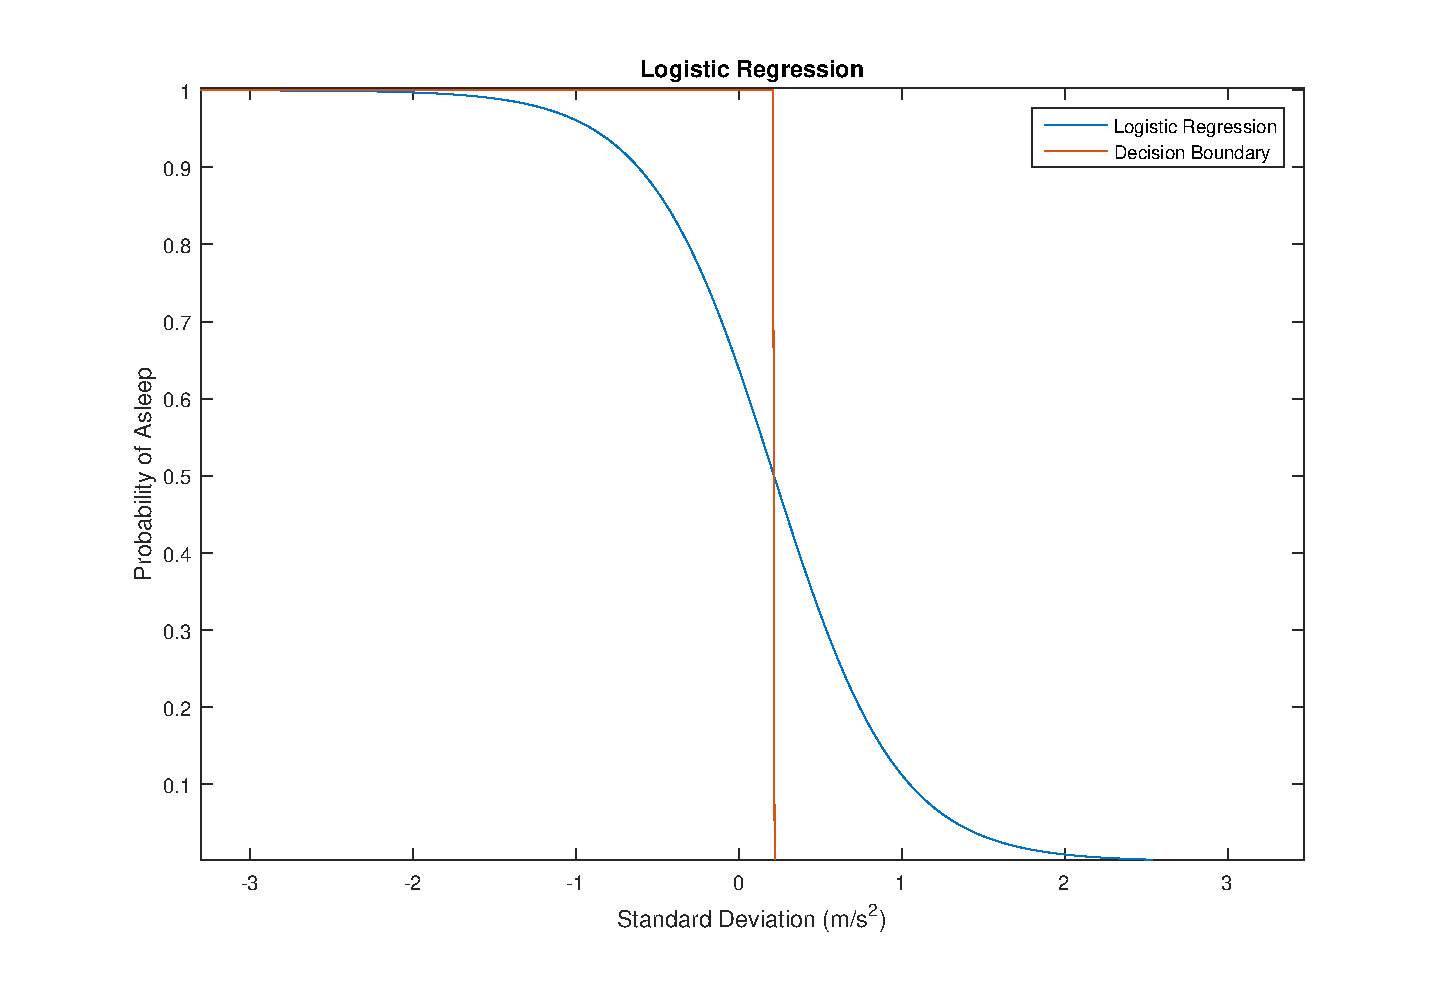
\includegraphics[width=0.75\textwidth]{Images/logistic_regression.eps}
                    \centering
                    \caption{A plot of the standard deviation of a signal segment against the probability of asleep. The step function represents the simplified decision boundary due to the single variable used.}
                    \label{img_regression}
                \end{figure}

                An example of the data under prediction can be seen below in Figure \ref{img_regression_ex}.

                \begin{figure}[h]
                    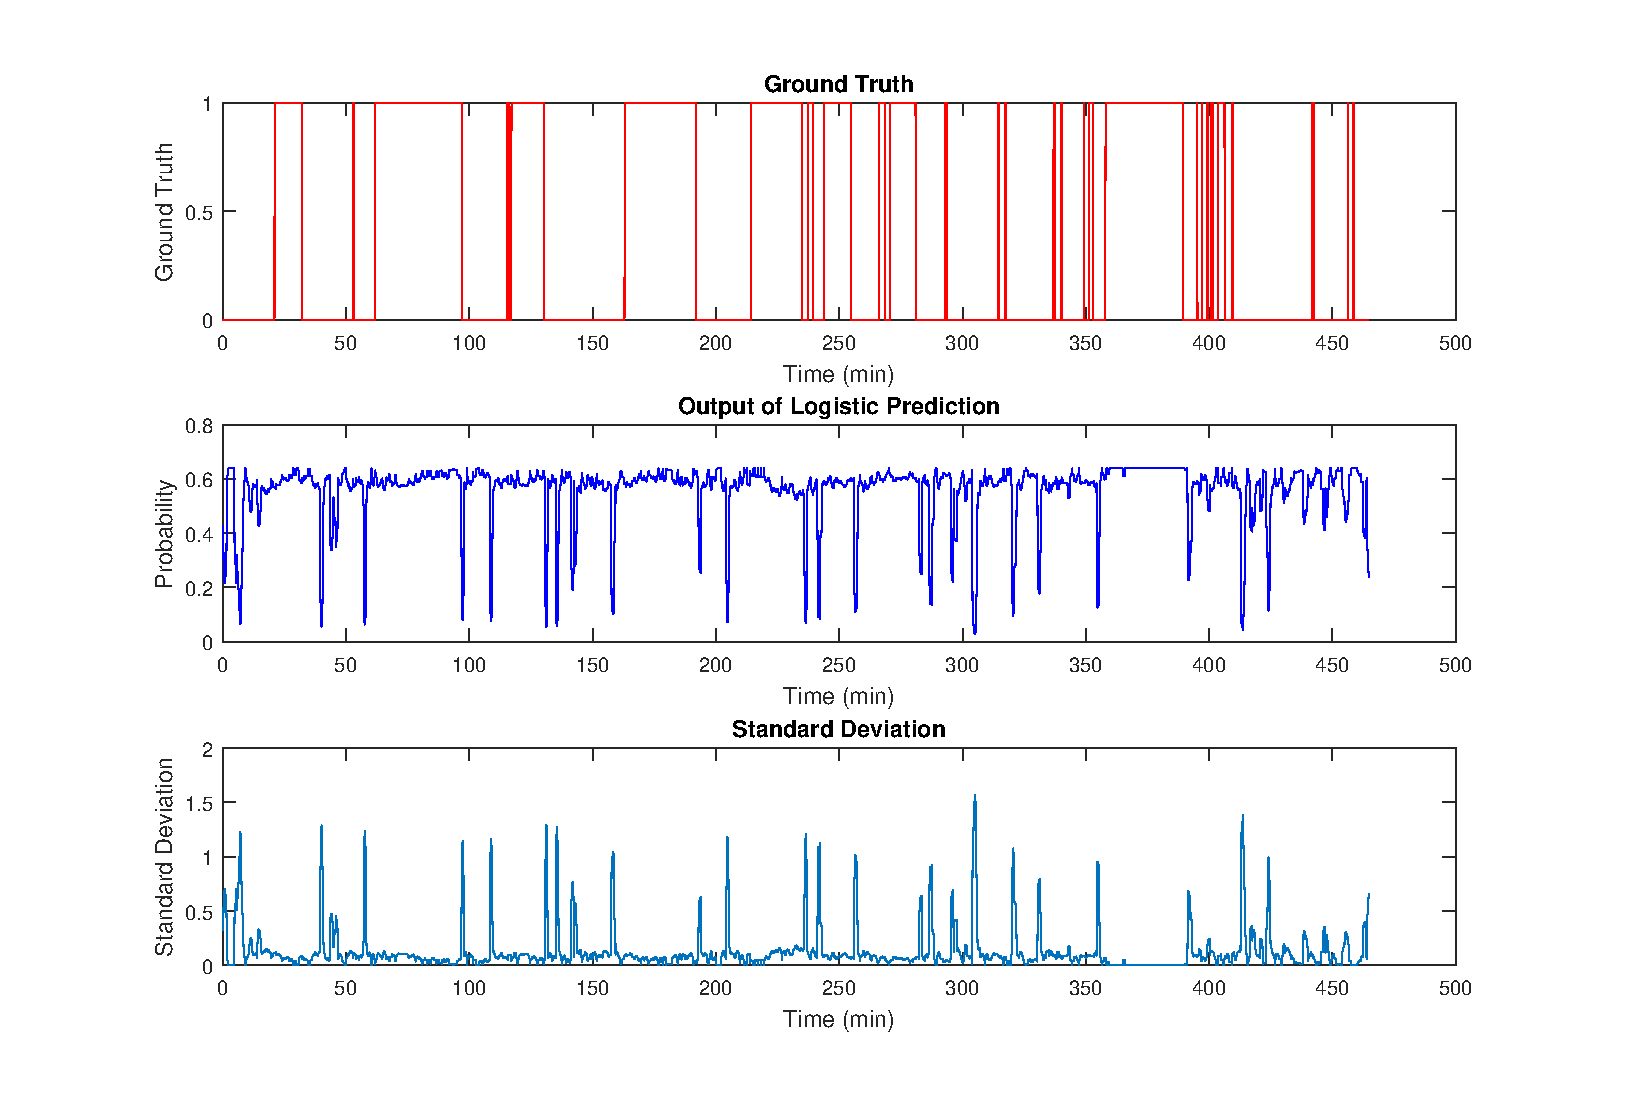
\includegraphics[width=0.8\textwidth]{Images/logistic_regression_ex.eps}
                    \centering
                    \caption{This is an example of the logistic regression making predictions based on standard deviation. Note how as standard deviation increase, the probability output decreases.}
                    \label{img_regression_ex}
                \end{figure}

        \section{Post-Prediction Filter}

            The next and final stage is a post-prediction filter. This stage exists due to the fact that classifying sleep for $100$ms periods is absurd for a detector based on an accelerometer signal. It is reasonable to assume that for our purposes, the minimum sleep time detectable is roughly $5$ minutes. This leads to the filter length discussed later on.

            The implementation of this filter works as a threshold, that is to say, if the output of the filter is above some value, the value gets rounded up and all other values get rounded down. This is to maintain the 0-1 classification inherent in the problem. 

            A window is taken around the point in question and the filter looks $k$ points to the left and $k$ points to the right of this point and the filter value is calculated by:

            \begin{equation}
                f_n = \sum_{i=-k}^k h_ix_{n+i}
            \end{equation}
            where $f_n$ is the filter value at the $n^{th}$ point, $h_i$ is the $i^{th}$ filter coefficient and $x_{n+i}$ is the $(x+i)_{th}$ point. If $f_n$ exceeds $t$, a chosen threshold, then the $n^{th}$ point is marked as asleep. $k$ is set to $1500$ for this filter, deriving from the $5$ minute minimum. 

            Two windows were considered for this filter: a moving average window (flat) and a Gaussian window. Each of these represents a different approach to the filter. The moving average window indicates that each point inside the window is valued equally, that is to say, the point $k$ timesteps away from the point under consideration is weighted the same as the point under consideration. The Gaussian windows is the opposite of this, points closer to the point under consideration are weighted more heavily than those farther away.

            A small script was written to select the best performing filter parameters: the threshold, $t$ would be varied for both filters from $0.85$ to $0.975$ at $0.025$ increments and the standard deviation, $\sigma$, for the Gaussian filter would be varied from $1000$ to $3500$ at $250$ increments. The threshold values were chosen in keeping with the idea that sleep will be fairly continuous along a signal, that is to say, the majority of datapoints should be positively classed as asleep in order to mark an area as asleep. The $\sigma$ values were chosen to align with the filter length of $3001$, this ensures that all values get a non-negligible weight, as filter coefficients at points outside of the $\begin{bmatrix}-2\sigma & 2\sigma \end{bmatrix}$ range are effectively given zero weighting.

            The best performing filter was the Gaussian with $t=0.975$ and $\sigma=2000$. An example of this post-prediction filter in action is shown below in Figure \ref{img_post_filter_ex}.

            \begin{figure}[h]
                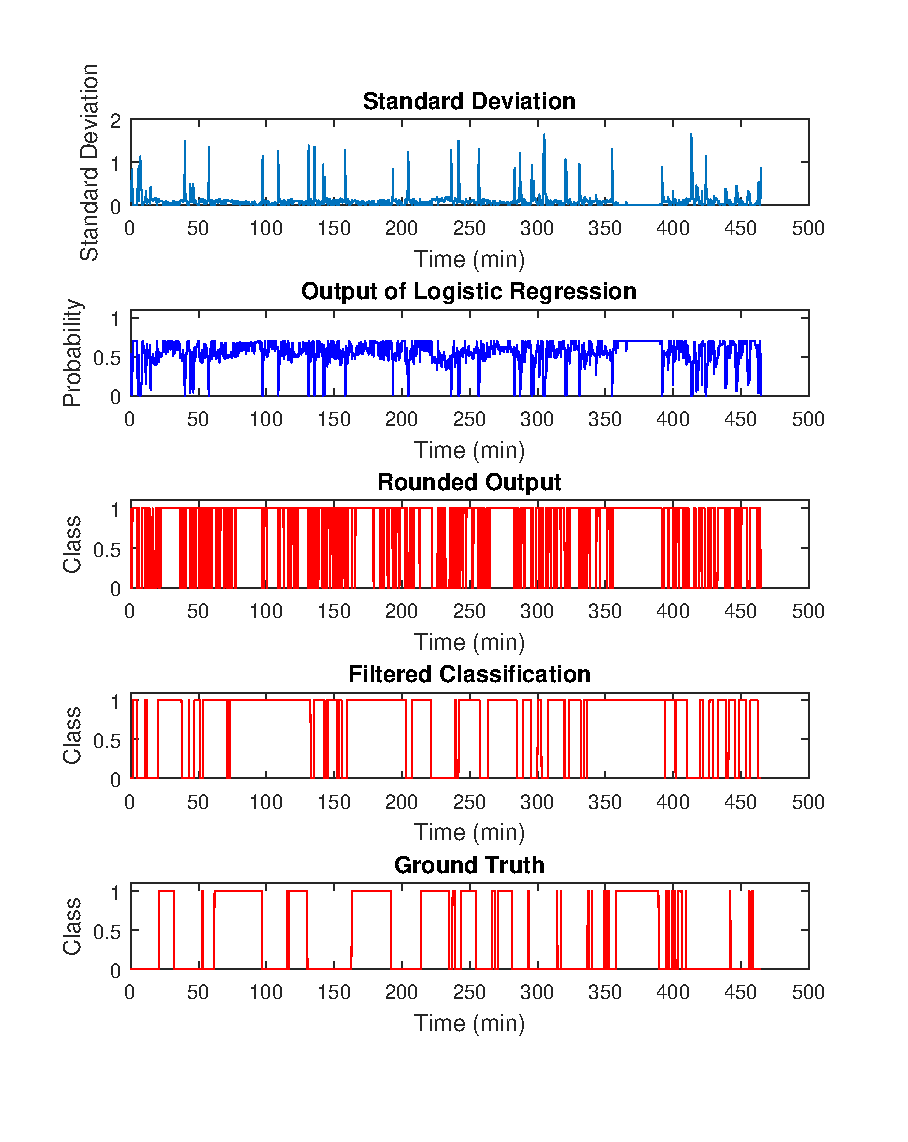
\includegraphics[width=0.8\textwidth]{Images/post_prediction_filters_ex.eps}
                \centering
                \caption{An example of the predicted output being filtered. The filter used was a Gaussian filter with length 3001 and standard deviation of 2000.}
                \label{img_post_filter_ex}
            \end{figure}


    \chapter{Results}

        The results presented here are a result of running the algorithm as described above, with no pre-prediction filter over $45$ of the $46$ data records in the Darmstadt database. One of the records was rejected as there was very little sleep in the record and the data was inconsistent throughout.

        An example of the algorithm classification in action can be seen in Figure \ref{img_ex_data_recording}. Note that a state of 1 indicates sleep, a state of 0 indicates wakefulness. 

        \begin{figure}[h]
            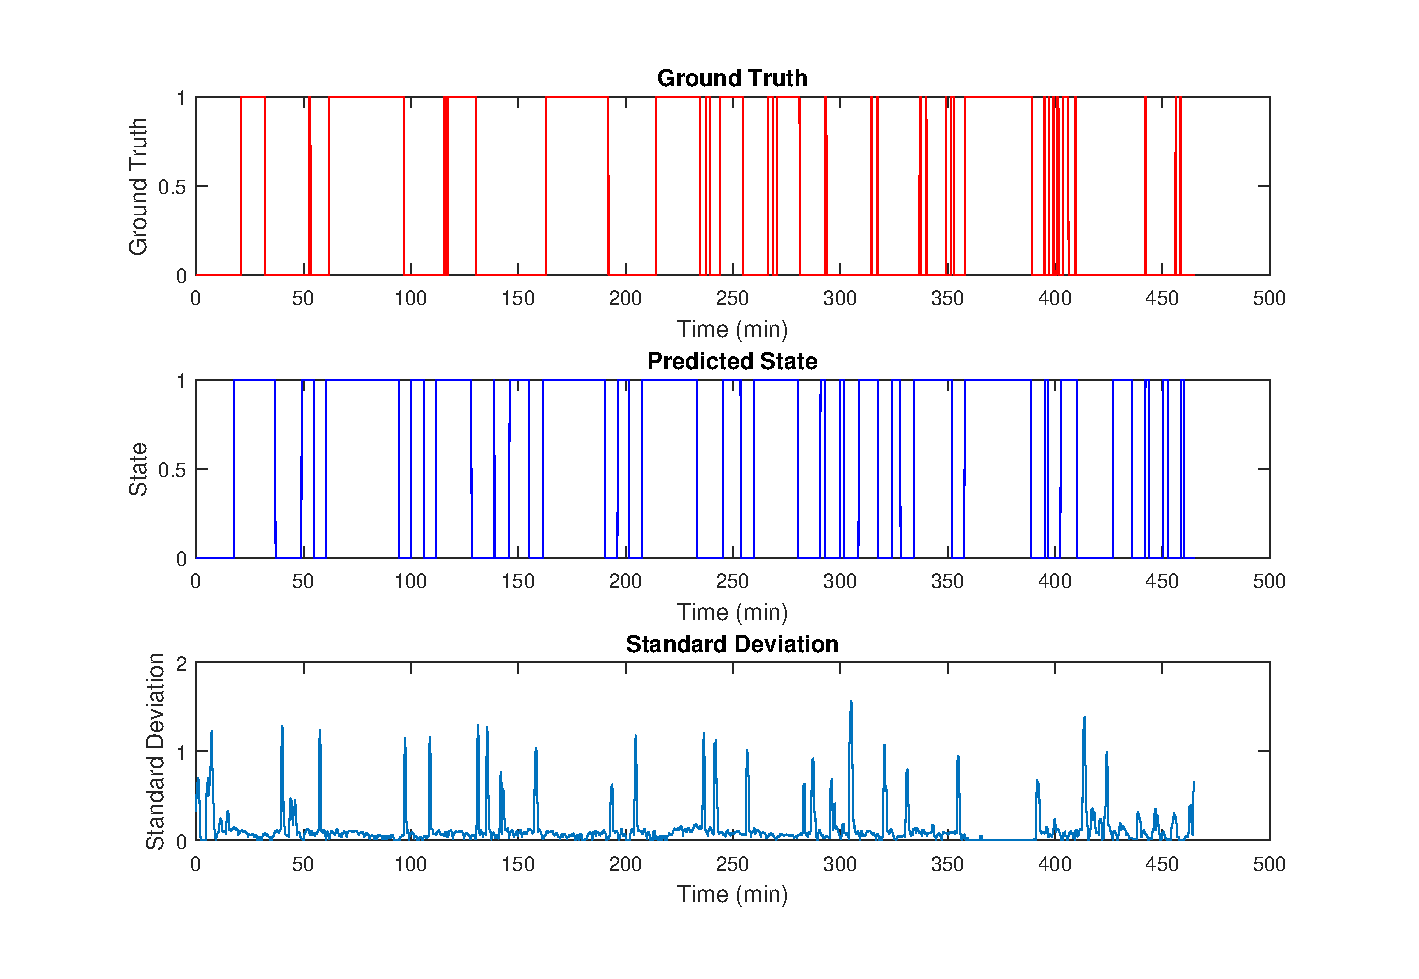
\includegraphics[width=\textwidth]{Images/example_data_recording.eps}
            \centering
            \caption{Example of the classification algorithm. From top to bottom: ground truth, predicted state, standard deviation.}
            \label{img_ex_data_recording}
        \end{figure}

        \section{Statistics}

            The algorithm is judged on 3 metrics: the Total Time Asleep (TTA), the total amount of sleeping time in the record, the Sleep Onset Time (SOT), the timestamp of the first incidence of sleep, and the Wakefulness Onset Time (WOT), the timestamp of the last incidence of sleep. The latter two parameters are representative of the start and end of a night's sleep. 

            For the algorithm described above, the following errors are achieved.

            \begin{center}
                \captionof{table}{Errors for the sleep detection algorithm.}
                \label{tbl_sleep_errors}
                \begin{tabular}{|c||c|c|}
                    \hline
                    Metric & Mean Error & Median Error \\
                    \hline
                    Total Time Asleep (\%) & 21.74\% & 11.89\% \\
                    Sleep Onset Time (minutes) & 25.08 min & 19.75 min \\
                    Wakefulness Onset Time (minutes) & 13.35 min & 3.86 min \\
                    \hline
                \end{tabular}
            \end{center}

            This performs better than the algorithm described in Borazio, et. al. [REF] that achieved 21.17\% median error for Total Time Asleep. This is almost a 10\% increase. The paper from Borazio, et. al. makes no mention of SOT or WOT statistics, so there can not be a comparison here.

            From the results, it is clear that all the error statistics have outliers far from the median since $e_{mean} > e_{median}$ for all the statistics. This is confirmed by the boxplots of the errors in Figures \ref{img_tta_error} and \ref{img_sot_wot_error}. For example, in the boxplot of TTA there are a number of outliers that skew the mean away from the median, but the bulk of the errors reside in between $0\%$ and $32\%$ error. 

            \begin{figure}[h]
                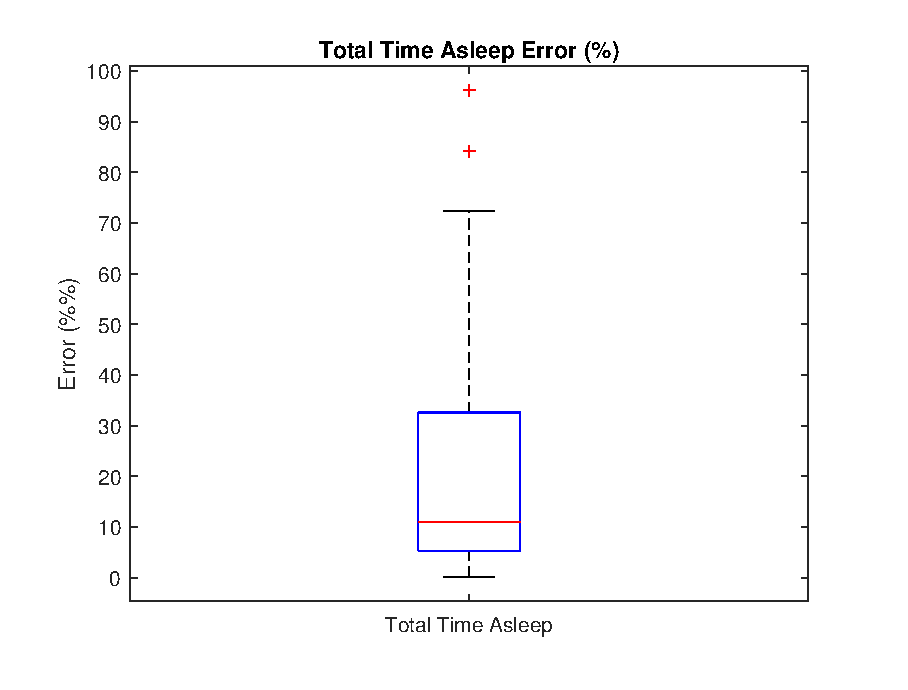
\includegraphics[width=0.75\textwidth]{Images/tta_error.eps}
                \centering
                \caption{Boxplot of errors for the Total Time Asleep. Median is at 11.89\%.}
                \label{img_tta_error}
            \end{figure}

            \begin{figure}[h]
                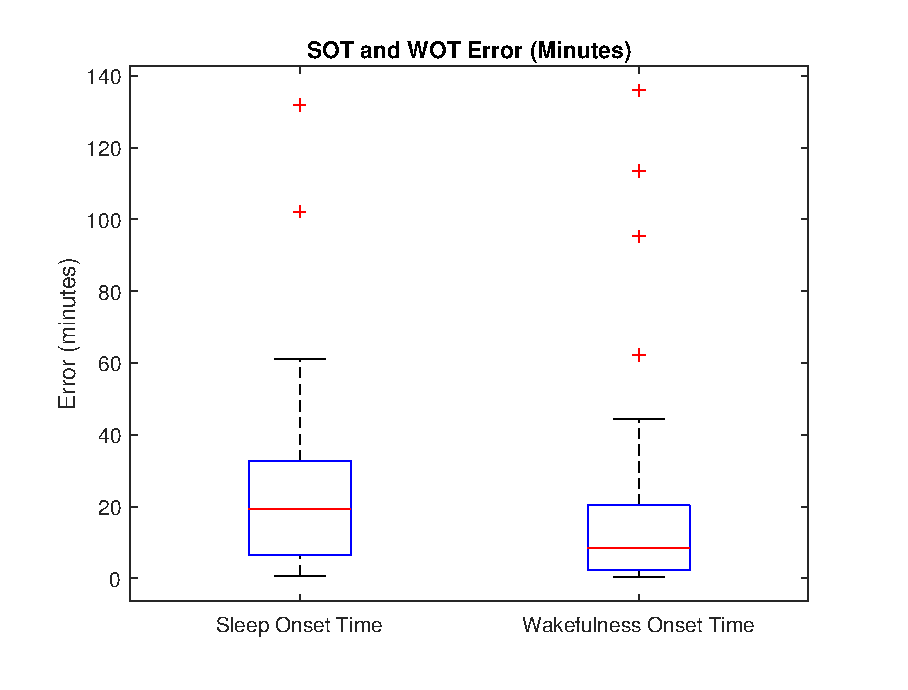
\includegraphics[width=0.75\textwidth]{Images/sot_wot_error.eps}
                \centering
                \caption{Boxplots of errors for the Sleep Onset Time and Wakefulness Onset Time. Note that the WOT is generally more accurate than the SOT.}
                \label{img_sot_wot_error}
            \end{figure}

            Another interesting thing is to examine the difference in accuracy between the SOT and WOT, as these fundamentally represent the two abilities of the algorithm: to identify sleep segments and to identify wakeful segments respectively. One explanation of the WOT being generally more accurate is that the end of sleep is generally very near to the end of the recording. So it could be a case of the recording ending limits the WOT error, whereas a similar phenomenom does not occur with the SOT.

        \section{Precision and Recall}

            A sensible way of quantifying these abilities is to look at the algorithm's precision and recall for both sleep states and awake states. Precision is defined as "the fraction of retrieved instances that are relevant" and recall is defined as "the fraction of relevant instances that are retrieved" [REF]. In this case, the sleep precision would be the percentage of predicted sleep states that are sleep states in the ground truth and the sleep recall would be the percentage of ground truth sleep states that were predicted sleep states. A similar description follows naturally for the wakeful states. The precision and recall were calculated on a per recording basis and tabulated for the entire algorithm. The results of this can be seen in Figure \ref{img_prec_recall}.

            \begin{figure}[h]
                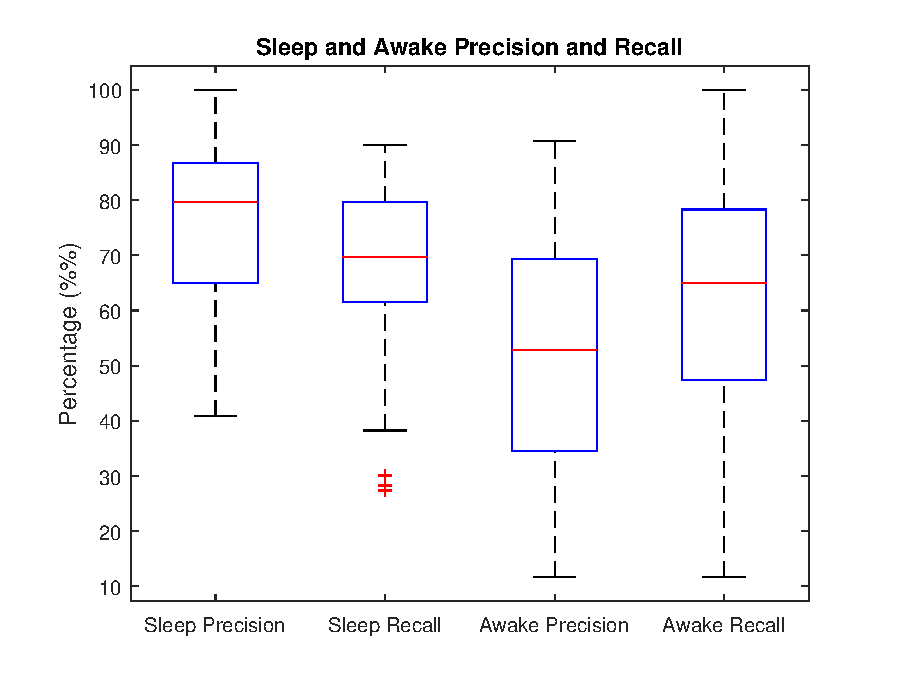
\includegraphics[width=0.75\textwidth]{Images/prec_recall.eps}
                \centering
                \caption{Boxplots of precision and recall for sleep and awake states. From left to right: sleep precision, sleep recall, awake precision, awake recall.}
                \label{img_prec_recall}
            \end{figure}

            The first thing to note is that the sleep precision is generally higher than that of awake. An explanation of this is that the algorithm is more biased toward classifying a point as awake than sleep. This means that the points that are classified as sleep are more likely to be sleep since the bar for classification is much for this. Another thing to note is that there is a very large variance in the awake precision and recall. This means that the algorithm generally had a hard time correctly identifying awake states. The awake recall being higher than precision indicates again that the algorithm tended to overclassify as awake. This is further supported by the recall of sleep being higher than the precision, also indicating that the algorithm is biased toward classifying as asleep. 

            This is interesting as in Borazio, et. al. the authors experienced the opposite case, along with the Cole [REF] and Oakley [REF] algorithms, in that they tended to overclassify as sleep. This is evidenced by the awake recall being much higher in this algorithm (65\% median vs. 45\% for Borazio, et. al.). This comes at the cost of a reduced sleep recall (70\% vs 94\% for Borazio, et. al.). Overall, this leads to a more balanced algorithm that is more equally adept at identifying sleep and awake states.


    \chapter{Further Work}

        Although small improvements were made to the sleep detector, there is still room for significant improvement. One area that can be explored is extending the feature vector used for prediction. Other features of the signal segment like the skewness or kurtosis of the distribution can be explored or examine the frequency content in the signal and attempt to correlate this with sleep states. Ultimately, this approach is limited due to the simple fact that it is impossible to discern the situation where someone is awake and not moving and the situation where someone is sleeping. One other area of interest is exploring extending the algorithm to include more sensors than the accelerometer like recording heartrate or the magnitude of light and using these factors as additional features. The structure of the algorithm is designed to accomodate additional features as these can simply be added to the feature vector without otherwise changing the algorithm.